\documentclass[11pt]{article}
\usepackage{graphicx}
\graphicspath{ {images/} }
\begin{document}

\begin{titlepage}

\begin{center}
\begin{huge}
Swarm Visualiser - COS 301 Main Project
\\
Functional Specification
\begin{small}
\\
Team: Dragon Brain
\\
Members:
\\
Matheu Botha u14284104
\\
Renton McInytre u14312710
\\
Emilio Singh u14006512
\\
Gerard van Wyk u14101263

\end{small}

\end{huge}
\end{center}
\end{titlepage}

\pagebreak

\tableofcontents

\pagebreak
\section{System Domain Model}
\paragraph{•}
In this section we will discuss and present a system-wide domain model and present the constituent systems, Modules, and their scopes

\begin{figure}[h]

\end{figure}
\section{Modules}
\subsection{General Optimiser}
\paragraph{•}
The General Optimiser or OPT for short is the module that provides the problem solving capacities of the system. It makes use of swarm-based methods to traverse user defined search spaces and perform evaluations of particles within the search space against user defined objective functions.
\subsubsection{Scope}
\paragraph{•}
The scope of the General Optimiser is presented below.
\begin{figure}[h]
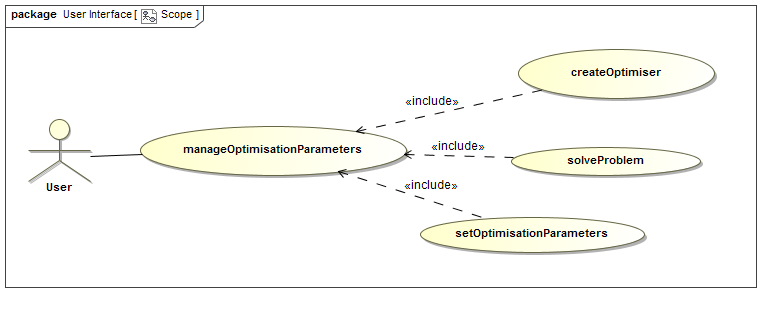
\includegraphics[scale=0.45]{Scope.png}
\end{figure}

\paragraph{•}
The User has 3 areas of general purpose use
\begin{itemize}
\item Creating Settings Packages which configure the Optimiser for runs
\item Changing Optimiser parameters during a run
\item Presenting problems for the Optimiser to solve
\end{itemize}
\subsubsection{Service Contracts}
\paragraph{•}
We will now specify the service contracts that importantly define the capacities of the General Optimiser Module

\subsubsection{Create Optimiser}
\begin{figure}[h]
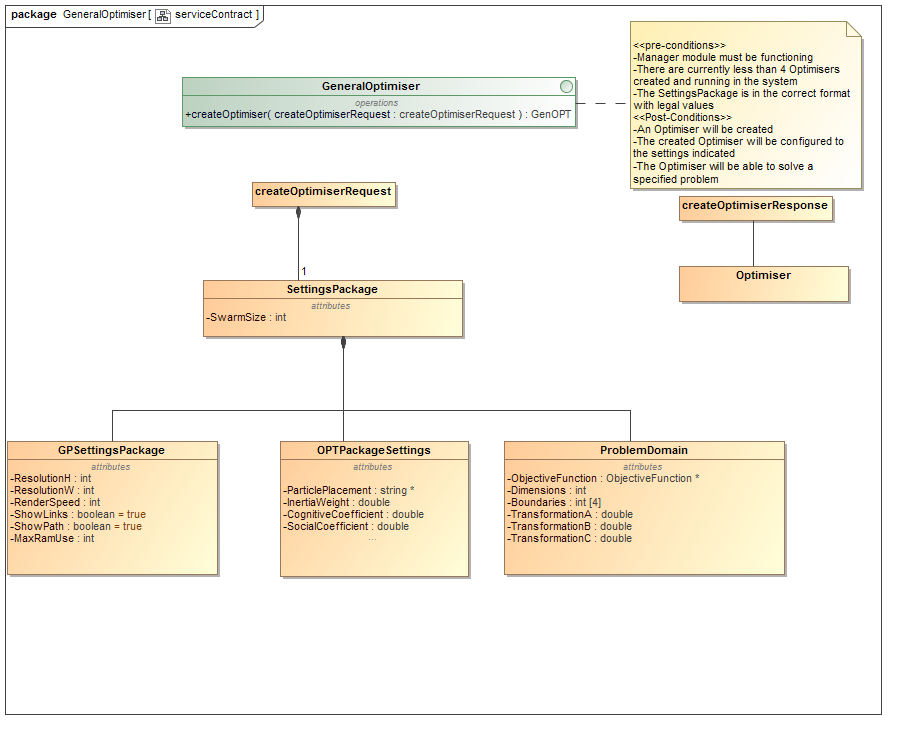
\includegraphics[scale=0.4]{serviceContractOPT.png}
\end{figure}

\paragraph{•}
The user will request for an Optimiser to be created. If there is space, that is less than 4 Optimisers already exist in the System, then the user will construct, indirectly, a SettingsPackage by entering their configuration parameters for the Optimiser. This Settings Package will be used by the Manager to construct and configure an Optimiser for use.

The exact conditions will be codified below:
\begin{enumerate}
\item There must be fewer than 4 Optimisers currently running in the system
\item The SettingsPackage received must contain specifications for all configuration parameters and must contain values for those parameters within legal domains.
\item The Manager Module is ready to receive/able to receive a new order/request from the User Interface.
\end{enumerate}

\subsubsection{Functional Requirements}
\begin{figure}[h]
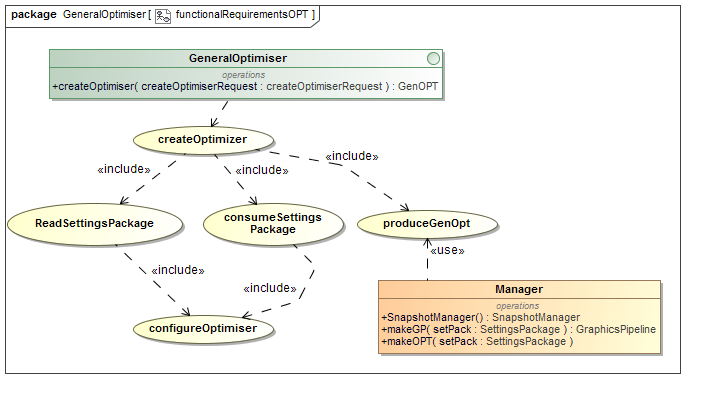
\includegraphics[scale=0.5]{functionalRequirementsOPT.png}
\end{figure}

\paragraph{•}
In terms of the functional requirements for the creation of an Optimiser object, a number of factors need to be considered in order for this to realised. Firstly, the reading and consumption of a Settings Package object relates to the process of extracting the necessary information from the settings package, the GenOPT package components, in order to provide the information during a constructor call. During the process, the Settings Package received is now invalidated and must be destroyed as it is at the end of its life-cycle. Once configuration has been completed, the GenOpt object will be produced and used by the Manager object.
\subsubsection{Process Design}
\paragraph{•}
The process specification defined here is for the process to create an Optimiser object.
\begin{figure}[h]
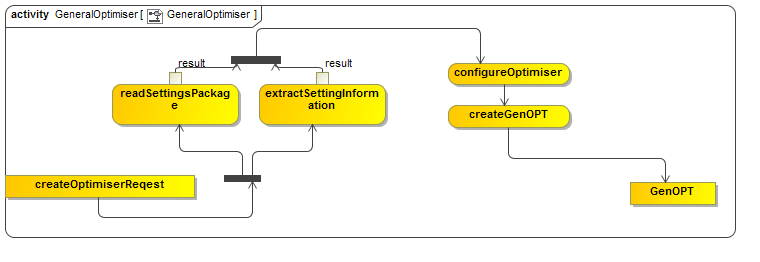
\includegraphics[scale=0.5]{GeneralOptimiserActivity.png}
\end{figure}

\subsubsection{Domain Model}
\paragraph{•}
Presented below is the domain model of the General Optimiser.
\begin{figure}[h]
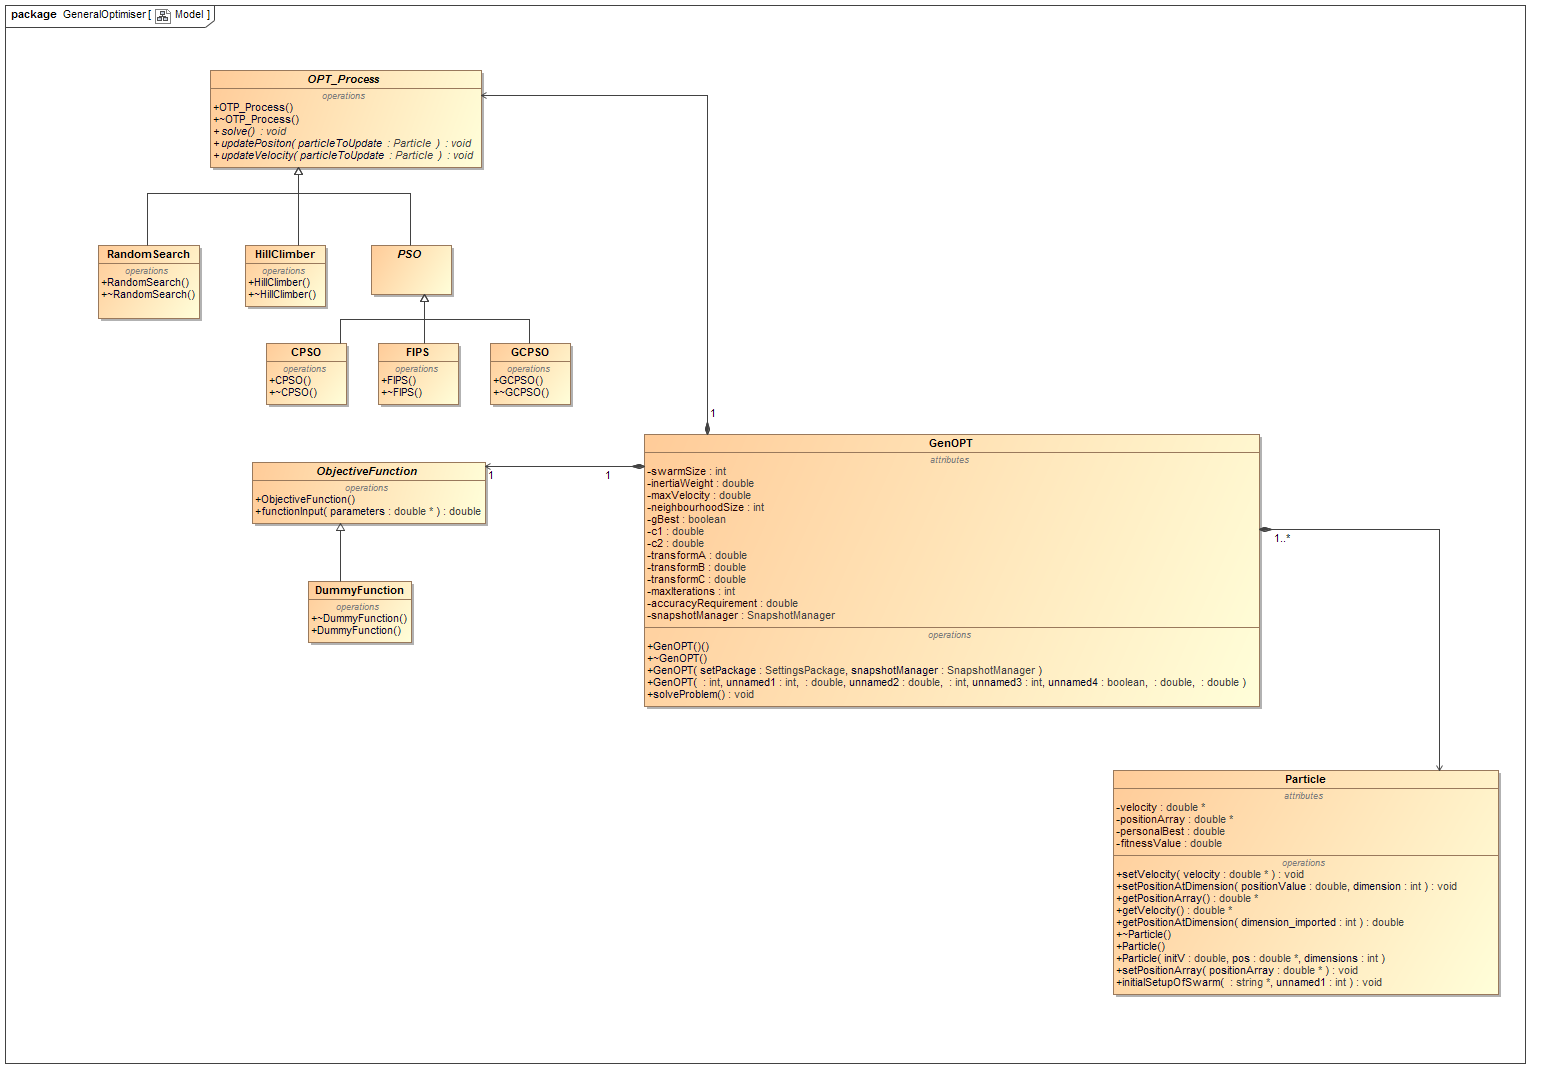
\includegraphics[scale=0.2]{OPTModel.png}
\end{figure}

\subsection{Graphics Processor}
The Graphics Processor is responsible for visualising the data that is generated by the Optimiser. 
\subsubsection{Scope}
The scope for the Graphics Processor is presented below: 
\subsubsection{Service Contracts}
\subsubsection{Functional Requirements}
\subsubsection{Process Design}

\subsection{Manager}
\subsubsection{Scope}
\subsubsection{Service Contracts}
\subsubsection{Functional Requirements}
\subsubsection{Process Design}

\subsection{User Interface}
\subsubsection{Scope}
The scope of the User Interface is presented below.
\begin{figure}[h]
	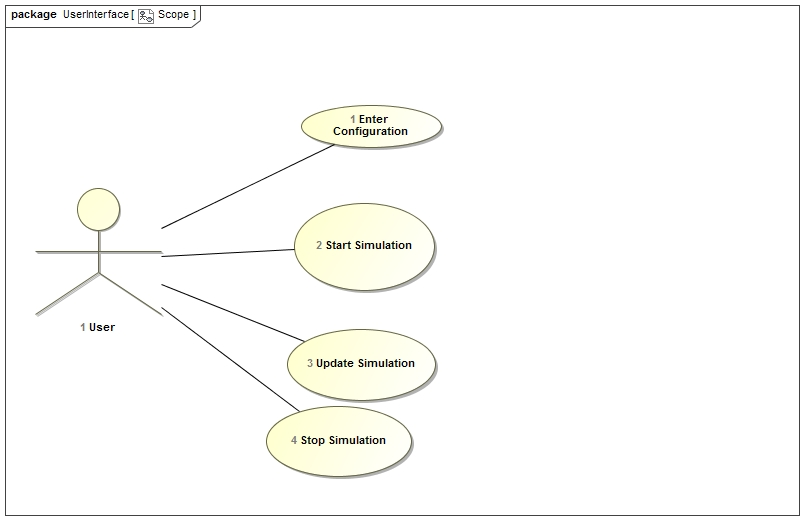
\includegraphics[scale=0.45]{GUI_Scope.png}
\end{figure}

\paragraph{•}
The User has 4 main capabilities
\begin{itemize}
	\item Changing the parameters of run environment
	\item Starting the simulation with the currently configured parameters.
	\item Updating the parameters of the current simulation based on the current (newly configured) parameters.
	\item Stopping the current simulation.
\end{itemize}

\subsubsection{Functional Requirements}
In terms of the Functional Requirements of the User Interface, the focus is as follows:
\begin{itemize}
	\item The user must be able to configure parameters for the system via the GUI.
	\item The GUI should be capable of sending data to the SettingsPackage in order to generate a SettingsPackage.
	\item The system should generate a SettingsPackage and start the simulation upon user request.
	\item The user should be able to edit configuration mid-run
\end{itemize}

\subsubsection{Activity Diagram}
Following is an activity diagram for the process involved in starting a run of the project.
\begin{figure}[h]
	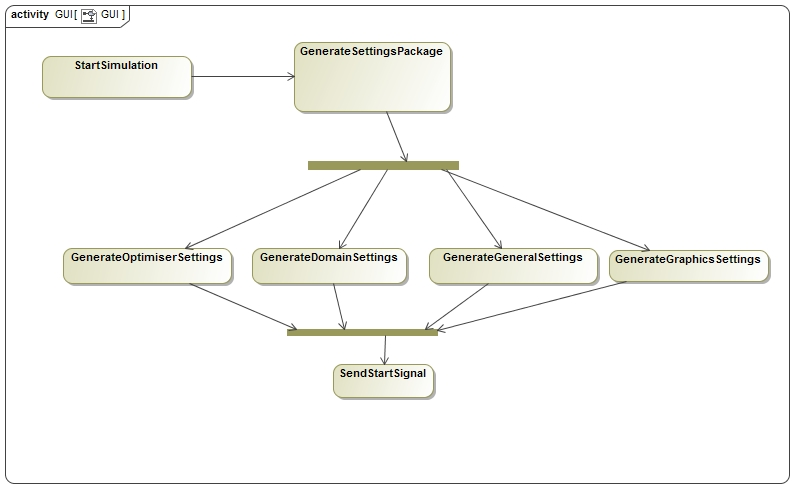
\includegraphics[scale=0.45]{GUI_Activity.png}
\end{figure}


\end{document}
